% vim:ft=tex:ts=2:sw=0:et
% Author: Plump Albert (plumpalbert@gmail.com)
\subsection{Диаграмма пакетов}
Диаграмма пакетов системы представлена на рисунке \ref{fig:diag-modules}.

\begin{figure}[H]
\centering
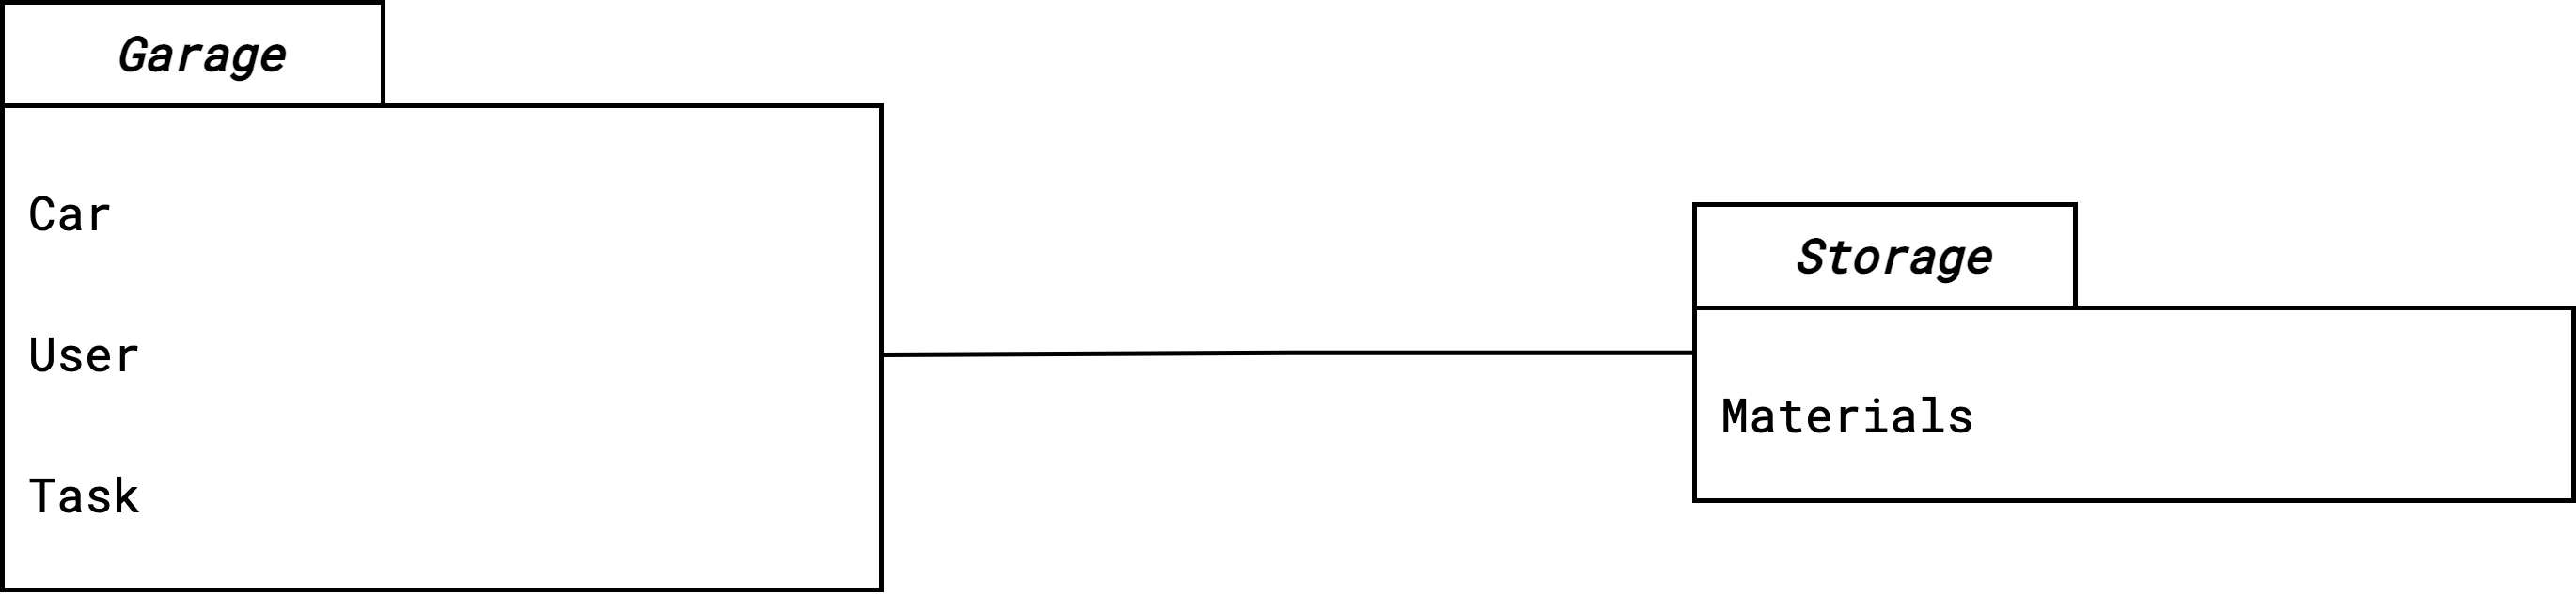
\includegraphics[keepaspectratio,width=\textwidth]{./images/diag-modules.png}
\caption{Диаграмма пакетов}
\label{fig:diag-modules}
\end{figure}

Спецификация пакетов представлена в таблицах \ref{tab:garage-module} --
\ref{tab:storage-module}.

\noindent\begin{longtblr}[
    caption = {Спецификация пакета \textquote{Garage}},
    label = tab:garage-module
  ]{
    hlines, vlines,
    colspec = {l l},
    width=\textwidth,
    rowhead=0,
    rowfoot=0
}
  Имя & Garage \\
  Стереотип & --- \\
  Зависимость & --- \\
  \SetCell[c=2]{l}{Список классов} \\
  \SetCell[c=2]{l}{Car, User, Task} \\
  \SetCell[c=2]{l}{Список пакетов} \\
  \SetCell[c=2]{l}{---} \\
  \SetCell[c=2]{l}{Описание} \\
  \SetCell[c=2]{l}
  Содержит сущности автомобилей, пользователей и задач ТО.
\end{longtblr}

\noindent\begin{longtblr}[
    caption = {Спецификация пакета \textquote{Storage}},
    label = tab:storage-module
  ]{
    hlines, vlines,
    colspec = {l l},
    width=\textwidth,
    rowhead=0,
    rowfoot=0
}
  Имя & Storage \\
  Стереотип & --- \\
  Зависимость & Garage \\
  \SetCell[c=2]{l}{Список классов} \\
  \SetCell[c=2]{l}{Materials} \\
  \SetCell[c=2]{l}{Список пакетов} \\
  \SetCell[c=2]{l}{---} \\
  \SetCell[c=2]{l}{Описание} \\
  \SetCell[c=2]{l}
  Содержит сущности материалов, хранящихся на складе организации.
\end{longtblr}
